\documentclass[a0paper]{tikzposter}
% Force a 16 by 9 ratio, 33.1 is same height as a0
\geometry{paperwidth=58.844in,paperheight=33.1in}

\makeatletter
\def\input@path{
  {../} % repository root
  {../latex-utilities} % LaTeX utilities
}
\makeatother

\usepackage{postertheme/vector_institute/vector_institute}

% \usepackage{amsmath}
\usepackage{amsmath,amssymb,mathtools,bm}
% requirements
\usepackage{amsmath}
\usepackage{amssymb}
\usepackage{bm}
\usepackage{mathtools}

% Random variables
\def\reta{{\textnormal{$\eta$}}}
\def\ra{{\textnormal{a}}}
\def\rb{{\textnormal{b}}}
\def\rc{{\textnormal{c}}}
\def\rd{{\textnormal{d}}}
\def\re{{\textnormal{e}}}
\def\rf{{\textnormal{f}}}
\def\rg{{\textnormal{g}}}
\def\rh{{\textnormal{h}}}
\def\ri{{\textnormal{i}}}
\def\rj{{\textnormal{j}}}
\def\rk{{\textnormal{k}}}
\def\rl{{\textnormal{l}}}
% rm is already a command, just don't name any random variables m
\def\rn{{\textnormal{n}}}
\def\ro{{\textnormal{o}}}
\def\rp{{\textnormal{p}}}
\def\rq{{\textnormal{q}}}
\def\rr{{\textnormal{r}}}
\def\rs{{\textnormal{s}}}
\def\rt{{\textnormal{t}}}
\def\ru{{\textnormal{u}}}
\def\rv{{\textnormal{v}}}
\def\rw{{\textnormal{w}}}
\def\rx{{\textnormal{x}}}
\def\ry{{\textnormal{y}}}
\def\rz{{\textnormal{z}}}

% Random vectors
\def\rvepsilon{{\mathbf{\epsilon}}}
\def\rvtheta{{\mathbf{\theta}}}
\def\rva{{\mathbf{a}}}
\def\rvb{{\mathbf{b}}}
\def\rvc{{\mathbf{c}}}
\def\rvd{{\mathbf{d}}}
\def\rve{{\mathbf{e}}}
\def\rvf{{\mathbf{f}}}
\def\rvg{{\mathbf{g}}}
\def\rvh{{\mathbf{h}}}
\def\rvu{{\mathbf{i}}}
\def\rvj{{\mathbf{j}}}
\def\rvk{{\mathbf{k}}}
\def\rvl{{\mathbf{l}}}
\def\rvm{{\mathbf{m}}}
\def\rvn{{\mathbf{n}}}
\def\rvo{{\mathbf{o}}}
\def\rvp{{\mathbf{p}}}
\def\rvq{{\mathbf{q}}}
\def\rvr{{\mathbf{r}}}
\def\rvs{{\mathbf{s}}}
\def\rvt{{\mathbf{t}}}
\def\rvu{{\mathbf{u}}}
\def\rvv{{\mathbf{v}}}
\def\rvw{{\mathbf{w}}}
\def\rvx{{\mathbf{x}}}
\def\rvy{{\mathbf{y}}}
\def\rvz{{\mathbf{z}}}

% Elements of random vectors
\def\erva{{\textnormal{a}}}
\def\ervb{{\textnormal{b}}}
\def\ervc{{\textnormal{c}}}
\def\ervd{{\textnormal{d}}}
\def\erve{{\textnormal{e}}}
\def\ervf{{\textnormal{f}}}
\def\ervg{{\textnormal{g}}}
\def\ervh{{\textnormal{h}}}
\def\ervi{{\textnormal{i}}}
\def\ervj{{\textnormal{j}}}
\def\ervk{{\textnormal{k}}}
\def\ervl{{\textnormal{l}}}
\def\ervm{{\textnormal{m}}}
\def\ervn{{\textnormal{n}}}
\def\ervo{{\textnormal{o}}}
\def\ervp{{\textnormal{p}}}
\def\ervq{{\textnormal{q}}}
\def\ervr{{\textnormal{r}}}
\def\ervs{{\textnormal{s}}}
\def\ervt{{\textnormal{t}}}
\def\ervu{{\textnormal{u}}}
\def\ervv{{\textnormal{v}}}
\def\ervw{{\textnormal{w}}}
\def\ervx{{\textnormal{x}}}
\def\ervy{{\textnormal{y}}}
\def\ervz{{\textnormal{z}}}

% Random matrices
\def\rmA{{\mathbf{A}}}
\def\rmB{{\mathbf{B}}}
\def\rmC{{\mathbf{C}}}
\def\rmD{{\mathbf{D}}}
\def\rmE{{\mathbf{E}}}
\def\rmF{{\mathbf{F}}}
\def\rmG{{\mathbf{G}}}
\def\rmH{{\mathbf{H}}}
\def\rmI{{\mathbf{I}}}
\def\rmJ{{\mathbf{J}}}
\def\rmK{{\mathbf{K}}}
\def\rmL{{\mathbf{L}}}
\def\rmM{{\mathbf{M}}}
\def\rmN{{\mathbf{N}}}
\def\rmO{{\mathbf{O}}}
\def\rmP{{\mathbf{P}}}
\def\rmQ{{\mathbf{Q}}}
\def\rmR{{\mathbf{R}}}
\def\rmS{{\mathbf{S}}}
\def\rmT{{\mathbf{T}}}
\def\rmU{{\mathbf{U}}}
\def\rmV{{\mathbf{V}}}
\def\rmW{{\mathbf{W}}}
\def\rmX{{\mathbf{X}}}
\def\rmY{{\mathbf{Y}}}
\def\rmZ{{\mathbf{Z}}}

% Elements of random matrices
\def\ermA{{\textnormal{A}}}
\def\ermB{{\textnormal{B}}}
\def\ermC{{\textnormal{C}}}
\def\ermD{{\textnormal{D}}}
\def\ermE{{\textnormal{E}}}
\def\ermF{{\textnormal{F}}}
\def\ermG{{\textnormal{G}}}
\def\ermH{{\textnormal{H}}}
\def\ermI{{\textnormal{I}}}
\def\ermJ{{\textnormal{J}}}
\def\ermK{{\textnormal{K}}}
\def\ermL{{\textnormal{L}}}
\def\ermM{{\textnormal{M}}}
\def\ermN{{\textnormal{N}}}
\def\ermO{{\textnormal{O}}}
\def\ermP{{\textnormal{P}}}
\def\ermQ{{\textnormal{Q}}}
\def\ermR{{\textnormal{R}}}
\def\ermS{{\textnormal{S}}}
\def\ermT{{\textnormal{T}}}
\def\ermU{{\textnormal{U}}}
\def\ermV{{\textnormal{V}}}
\def\ermW{{\textnormal{W}}}
\def\ermX{{\textnormal{X}}}
\def\ermY{{\textnormal{Y}}}
\def\ermZ{{\textnormal{Z}}}

% Vectors
\def\vzero{{\bm{0}}}
\def\vone{{\bm{1}}}
\def\vmu{{\bm{\mu}}}
\def\vnu{{\bm{\nu}}}
\def\vtheta{{\bm{\theta}}}
\def\vepsilon{{\bm{\epsilon}}}
\def\vgamma{{\bm{\gamma}}}
\def\vdelta{{\bm{\delta}}}
\def\vDelta{{\bm{\Delta}}}
\def\va{{\bm{a}}}
\def\vb{{\bm{b}}}
\def\vc{{\bm{c}}}
\def\vd{{\bm{d}}}
\def\ve{{\bm{e}}}
\def\vetilde{\bm{\tilde{e}}}
\def\vell{{\bm{\ell}}}
\def\vf{{\bm{f}}}
\def\vg{{\bm{g}}}
\def\vh{{\bm{h}}}
\def\vi{{\bm{i}}}
\def\vj{{\bm{j}}}
\def\vk{{\bm{k}}}
\def\vl{{\bm{l}}}
\def\vm{{\bm{m}}}
\def\vmhat{{\bm{\hat{m}}}}
\def\vn{{\bm{n}}}
\def\vo{{\bm{o}}}
\def\vp{{\bm{p}}}
\def\vphi{{\bm{\phi}}}
\def\vq{{\bm{q}}}
\def\vr{{\bm{r}}}
\def\vs{{\bm{s}}}
\def\vstilde{\bm{\tilde{s}}}
\def\vt{{\bm{t}}}
\def\vu{{\bm{u}}}
\def\vv{{\bm{v}}}
\def\vvhat{{\bm{\hat{v}}}}
\def\vw{{\bm{w}}}
\def\vx{{\bm{x}}}
\def\vy{{\bm{y}}}
\def\vytilde{{\bm{\tilde{y}}}}
\def\vyhat{{\bm{\hat{y}}}}
\def\vz{{\bm{z}}}

% Elements of vectors
\def\evalpha{{\alpha}}
\def\evbeta{{\beta}}
\def\evepsilon{{\epsilon}}
\def\evlambda{{\lambda}}
\def\evomega{{\omega}}
\def\evmu{{\mu}}
\def\evpsi{{\psi}}
\def\evsigma{{\sigma}}
\def\evtheta{{\theta}}
\def\eva{{a}}
\def\evb{{b}}
\def\evc{{c}}
\def\evd{{d}}
\def\eve{{e}}
\def\evf{{f}}
\def\evg{{g}}
\def\evh{{h}}
\def\evi{{i}}
\def\evj{{j}}
\def\evk{{k}}
\def\evl{{l}}
\def\evm{{m}}
\def\evn{{n}}
\def\evo{{o}}
\def\evp{{p}}
\def\evq{{q}}
\def\evr{{r}}
\def\evs{{s}}
\def\evt{{t}}
\def\evu{{u}}
\def\evv{{v}}
\def\evw{{w}}
\def\evx{{x}}
\def\evy{{y}}
\def\evyhat{{\hat{y}}}
\def\evz{{z}}

% Matrix
\def\mA{{\bm{A}}}
\def\mB{{\bm{B}}}
\def\mC{{\bm{C}}}
\def\mD{{\bm{D}}}
\def\mE{{\bm{E}}}
\def\mF{{\bm{F}}}
\def\mG{{\bm{G}}}
\def\mGtilde{\bm{\tilde{G}}}
\def\mH{{\bm{H}}}
\def\mI{{\bm{I}}}
\def\mJ{{\bm{J}}}
\def\mK{{\bm{K}}}
\def\mL{{\bm{L}}}
\def\mM{{\bm{M}}}
\def\mN{{\bm{N}}}
\def\mO{{\bm{O}}}
\def\mP{{\bm{P}}}
\def\mQ{{\bm{Q}}}
\def\mR{{\bm{R}}}
\def\mS{{\bm{S}}}
\def\mT{{\bm{T}}}
\def\mU{{\bm{U}}}
\def\mV{{\bm{V}}}
\def\mW{{\bm{W}}}
\def\mX{{\bm{X}}}
\def\mY{{\bm{Y}}}
\def\mZ{{\bm{Z}}}
\def\mBeta{{\bm{\beta}}}
\def\mGamma{{\bm{\Gamma}}}
\def\mPhi{{\bm{\Phi}}}
\def\mPi{{\bm{\Pi}}}
\def\mLambda{{\bm{\Lambda}}}
\def\mSigma{{\bm{\Sigma}}}
\def\mOmega{{\bm{\Omega}}}
\def\mStilde{\bm{\tilde{\mS}}}
\def\mGtilde{\bm{\tilde{\mG}}}
\def\mGoverline{{\bm{\overline{G}}}}

% Tensor
\DeclareMathAlphabet{\mathsfit}{\encodingdefault}{\sfdefault}{m}{sl}
\SetMathAlphabet{\mathsfit}{bold}{\encodingdefault}{\sfdefault}{bx}{n}
\newcommand{\tens}[1]{\bm{\mathsfit{#1}}}
\def\tA{{\tens{A}}}
\def\tB{{\tens{B}}}
\def\tC{{\tens{C}}}
\def\tD{{\tens{D}}}
\def\tE{{\tens{E}}}
\def\tF{{\tens{F}}}
\def\tG{{\tens{G}}}
\def\tH{{\tens{H}}}
\def\tI{{\tens{I}}}
\def\tJ{{\tens{J}}}
\def\tK{{\tens{K}}}
\def\tL{{\tens{L}}}
\def\tM{{\tens{M}}}
\def\tN{{\tens{N}}}
\def\tO{{\tens{O}}}
\def\tP{{\tens{P}}}
\def\tPi{\bm{\mathsf{\Pi}}}
\def\tQ{{\tens{Q}}}
\def\tR{{\tens{R}}}
\def\tS{{\tens{S}}}
\def\tT{{\tens{T}}}
\def\tU{{\tens{U}}}
\def\tV{{\tens{V}}}
\def\tW{{\tens{W}}}
\def\tX{{\tens{X}}}
\def\tY{{\tens{Y}}}
\def\tZ{{\tens{Z}}}

% Graph
\def\gA{{\mathcal{A}}}
\def\gB{{\mathcal{B}}}
\def\gC{{\mathcal{C}}}
\def\gD{{\mathcal{D}}}
\def\gE{{\mathcal{E}}}
\def\gF{{\mathcal{F}}}
\def\gG{{\mathcal{G}}}
\def\gH{{\mathcal{H}}}
\def\gI{{\mathcal{I}}}
\def\gJ{{\mathcal{J}}}
\def\gK{{\mathcal{K}}}
\def\gL{{\mathcal{L}}}
\def\gM{{\mathcal{M}}}
\def\gN{{\mathcal{N}}}
\def\gO{{\mathcal{O}}}
\def\gP{{\mathcal{P}}}
\def\gQ{{\mathcal{Q}}}
\def\gR{{\mathcal{R}}}
\def\gS{{\mathcal{S}}}
\def\gT{{\mathcal{T}}}
\def\gU{{\mathcal{U}}}
\def\gV{{\mathcal{V}}}
\def\gW{{\mathcal{W}}}
\def\gX{{\mathcal{X}}}
\def\gY{{\mathcal{Y}}}
\def\gZ{{\mathcal{Z}}}

% Sets
\def\sA{{\mathbb{A}}}
\def\sB{{\mathbb{B}}}
\def\sC{{\mathbb{C}}}
\def\sD{{\mathbb{D}}}
% Don't use a set called E, because this would be the same as our symbol
% for expectation.
\def\sF{{\mathbb{F}}}
\def\sG{{\mathbb{G}}}
\def\sH{{\mathbb{H}}}
\def\sI{{\mathbb{I}}}
\def\sJ{{\mathbb{J}}}
\def\sK{{\mathbb{K}}}
\def\sL{{\mathbb{L}}}
\def\sM{{\mathbb{M}}}
\def\sN{{\mathbb{N}}}
\def\sO{{\mathbb{O}}}
\def\sP{{\mathbb{P}}}
\def\sQ{{\mathbb{Q}}}
\def\sR{{\mathbb{R}}}
\def\sS{{\mathbb{S}}}
\def\sT{{\mathbb{T}}}
\def\sU{{\mathbb{U}}}
\def\sV{{\mathbb{V}}}
\def\sW{{\mathbb{W}}}
\def\sX{{\mathbb{X}}}
\def\sY{{\mathbb{Y}}}
\def\sYhat{{\hat{\mathbb{Y}}}}
\def\sZ{{\mathbb{Z}}}
% Blackboard Greek characters: https://tex.stackexchange.com/a/3260
\DeclareSymbolFont{bbold}{U}{bbold}{m}{n}
\DeclareSymbolFontAlphabet{\mathbbold}{bbold}
\def\sTheta{{\mathbbold{\Theta}}}
\def\sOmega{{\mathbbold{\Omega}}}

% Entries of a matrix
\def\emLambda{{\Lambda}}
\def\emA{{A}}
\def\emB{{B}}
\def\emC{{C}}
\def\emD{{D}}
\def\emE{{E}}
\def\emF{{F}}
\def\emG{{G}}
\def\emH{{H}}
\def\emI{{I}}
\def\emJ{{J}}
\def\emK{{K}}
\def\emL{{L}}
\def\emM{{M}}
\def\emN{{N}}
\def\emO{{O}}
\def\emP{{P}}
\def\emQ{{Q}}
\def\emR{{R}}
\def\emS{{S}}
\def\emT{{T}}
\def\emU{{U}}
\def\emV{{V}}
\def\emW{{W}}
\def\emX{{X}}
\def\emY{{Y}}
\def\emZ{{Z}}
\def\emSigma{{\Sigma}}
\def\emPi{{\Pi}}

% entries of a tensor
% Same font as tensor, without \bm wrapper
\newcommand{\etens}[1]{\mathsfit{#1}}
\def\etLambda{{\etens{\Lambda}}}
\def\etA{{\etens{A}}}
\def\etB{{\etens{B}}}
\def\etC{{\etens{C}}}
\def\etD{{\etens{D}}}
\def\etE{{\etens{E}}}
\def\etF{{\etens{F}}}
\def\etG{{\etens{G}}}
\def\etH{{\etens{H}}}
\def\etI{{\etens{I}}}
\def\etJ{{\etens{J}}}
\def\etK{{\etens{K}}}
\def\etL{{\etens{L}}}
\def\etM{{\etens{M}}}
\def\etN{{\etens{N}}}
\def\etO{{\etens{O}}}
\def\etP{{\etens{P}}}
\def\etPi{\mathsf{\Pi}}
\def\etQ{{\etens{Q}}}
\def\etR{{\etens{R}}}
\def\etS{{\etens{S}}}
\def\etT{{\etens{T}}}
\def\etU{{\etens{U}}}
\def\etV{{\etens{V}}}
\def\etW{{\etens{W}}}
\def\etX{{\etens{X}}}
\def\etY{{\etens{Y}}}
\def\etZ{{\etens{Z}}}

% The true underlying data generating distribution
\newcommand{\pdata}{p_{\mathrm{data}}}
% The empirical distribution defined by the training set
\newcommand{\ptrain}{\hat{p}_{\mathrm{data}}}
\newcommand{\Ptrain}{\hat{P}_{\mathrm{data}}}
% The model distribution
\newcommand{\pmodel}{p_{\rm{model}}}
\newcommand{\Pmodel}{P_{\rm{model}}}
\newcommand{\ptildemodel}{\tilde{p}_{\rm{model}}}
% Stochastic autoencoder distributions
\newcommand{\pencode}{p_{\rm{encoder}}}
\newcommand{\pdecode}{p_{\rm{decoder}}}
\newcommand{\precons}{p_{\rm{reconstruct}}}

\newcommand{\laplace}{\mathrm{Laplace}} % Laplace distribution

\newcommand{\E}{\mathbb{E}}
\newcommand{\Ls}{\mathcal{L}}
\newcommand{\R}{\mathbb{R}}
\newcommand{\emp}{\tilde{p}}
\newcommand{\lr}{\alpha}
\newcommand{\reg}{\lambda}
\newcommand{\rect}{\mathrm{rectifier}}
\newcommand{\softmax}{\mathrm{softmax}}
\newcommand{\onehot}{\mathrm{onehot}}
\newcommand{\sigmoid}{\sigma}
\newcommand{\softplus}{\zeta}
\newcommand{\KL}{D_{\mathrm{KL}}}
\newcommand{\Var}{\mathrm{Var}}
\newcommand{\standarderror}{\mathrm{SE}}
\newcommand{\Cov}{\mathrm{Cov}}
% Wolfram Mathworld says $L^2$ is for function spaces and $\ell^2$ is for vectors
% But then they seem to use $L^2$ for vectors throughout the site, and so does
% wikipedia.
\newcommand{\normlzero}{L^0}
\newcommand{\normlone}{L^1}
\newcommand{\normltwo}{L^2}
\newcommand{\normlp}{L^p}
\newcommand{\normmax}{L^\infty}

\newcommand{\parents}{Pa} % See usage in notation.tex. Chosen to match Daphne's book.

\DeclareMathOperator*{\argmax}{arg\,max}
\DeclareMathOperator*{\argmin}{arg\,min}
\DeclareMathOperator*{\minimize}{minimize}
\DeclareMathOperator*{\maximize}{maximize}

\DeclareMathOperator{\sign}{sign}
\DeclareMathOperator{\mean}{mean}
\DeclareMathOperator{\vmap}{vmap}
\DeclareMathOperator{\reshape}{reshape}
\DeclareMathOperator{\Tr}{Tr}
\DeclareMathOperator{\diag}{diag}
\DeclareMathOperator{\eig}{eig}
\DeclareMathOperator{\rank}{rank}
\DeclareMathOperator{\vecspan}{span}
\DeclareMathOperator{\overlap}{overlap}
\DeclareMathOperator{\Cat}{Cat}
\DeclareMathOperator{\flatten}{vec}
\DeclareMathOperator{\blockdiag}{blockdiag}

%%%%% NEW MATH DEFINITIONS %%%%%
\newcommand{\jac}{\mathrm{J}}
\newcommand{\grad}[1]{\ensuremath{\nabla_{\!{#1}}}}
\newcommand{\gradsquared}[1]{\ensuremath{\nabla_{\!{#1}}^{2}}}

% || for KLDivergence
\DeclarePairedDelimiterX{\KLdivx}[2]{(}{)}{%
  #1\;\delimsize\|\;#2%
}
\newcommand{\KLdiv}{\KL\KLdivx}

% | for a | b
\newcommand{\giventhat}[2]{#1\;|\;#2}

\let\ab\allowbreak
%%% Local Variables:
%%% mode: latex
%%% TeX-master: "../main"
%%% End:

% math in sans serif
\usepackage{sfmath}

\usetikzlibrary{arrows.meta}

% \useblockstyle{Envelope}
% \usebackgroundstyle{Empty}
\usetitlestyle{Filled}

\title{
  \fontsize{115}{60}\selectfont
  \bf Kronecker-Factored Approximate Curvature
  for Physics-Informed Neural Networks}
\author{\Huge
  Felix Dangel*, Johannes M\"uller*, Marius Zeinhofer*
}
\institute{
  \LARGE
  Vector Institute (Canada), RWTH Aachen University (Germany), Simula Research Laboratory (Norway)
}


\begin{document}
% ==============================================================================
% HEADER & FOOTER

\backgroundgradient % Adds the background features
\maketitle
\headerlogo % Adds Vector logo to header
\posterfooter{
  % Poster footer with additional information
} % Footer

\hspace{-35cm}
\begin{columns}
  \centering
  \begin{column}{1.85}
    \centering \ribbon{\centering\fontsize{105}{80}\selectfont\textcolor{white}{\bf
        We develop KFAC for loss functions with differential operators.
        \\[0.5ex]
        For training PINNs, our optimizer consistently outperforms SGD/Adam.
        % We generalize KFAC to PINN losses (which contain differential operators) \\
        % using Taylor-mode autodiff and the concept of linear weight sharing layers.
      }}
  \end{column}
\end{columns}
\hspace{2cm}

\begin{columns}
  \column{0.9}
  \block{Background: What Are PINNs?}{
    \begin{Large}
      \begin{center}
        \textcolor{VectorBlue}{\textbf{Main idea: Train a neural network to satisfy a PDE $\to$ loss contains the PDE's differential operator.}}
      \end{center}
    \end{Large}

    \vspace{1ex}

    \begin{minipage}[t]{0.4\linewidth}
      \begin{itemize}
      \item \textbf{Goal:} Learn PDE solution $u(\vx)$
        \begin{align*}
          \gL u(\vx) &= f(\vx) \qquad  \vx \in \Omega
          \\
          u(\vx) &= g(\vx) \qquad  \vx \in \partial\Omega
        \end{align*}

      \item \textbf{Example:} 2d Poisson equation
        \begin{align*}
          \gL = \frac{\partial^2}{\partial x_1^2} + \frac{\partial^2}{\partial x_2^2}
        \end{align*}
      \end{itemize}

    \end{minipage}
    \hfill
    \begin{minipage}[t]{0.6\linewidth}
      \begin{itemize}
      \item \textbf{Data:} Sample $\vx_n \sim \Omega$, $\vx_n^{\text{b}} \sim \partial \Omega$

      \item \textbf{Ansatz:} Neural net $u_{\vtheta}(\vx)$
        \begin{align*}
          L(\vtheta)
          =
          \underbrace{
          \frac{1}{2N_{\Omega}} \sum_{n=1}^{N_{\Omega}}
          \left(
          \gL u_{\vtheta}(\vx_n) - f(\vx_n)
          \right)^2
          }_{\substack{
          L_{\Omega}(\vtheta)
          \\[1ex] \textbf{\large satisfy interior condition}
          }}
          +
          \underbrace{
          \frac{1}{2N_{\partial\Omega}} \sum_{n=1}^{N_{\partial\Omega}}
          \left(
          u_{\vtheta}(\vx_n^{\text{b}}) - g(\vx_n^{\text{b}})
          \right)^2
          }_{\substack{
          L_{\partial\Omega}(\vtheta)
          \\[1ex] \textbf{\large satisfy boundary condition}
          }}
        \end{align*}
      \end{itemize}
    \end{minipage}

    \vspace{1ex}

    \begin{minipage}{0.33\linewidth}
      \centering
      % [trim={left bottom right top},clip]
      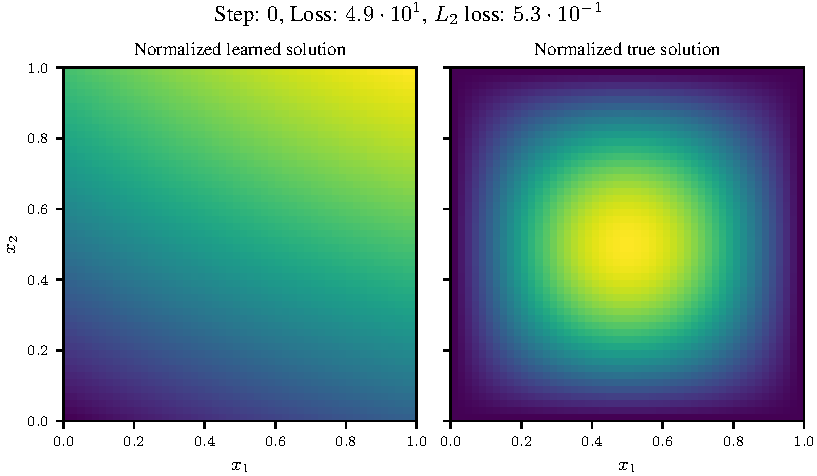
\includegraphics[scale=2,trim={0.9cm 0.8cm 6.7cm 1cm}, clip]{../kfac_pinns_exp/exp42_visualize_solutions/visualize_solution/SGD/poisson_2d_sin_product_mlp-tanh-64_SGD_step0000000.pdf}

      \textbf{Untrained}
    \end{minipage}
    \hfill
    \begin{minipage}{0.33\linewidth}
      \centering
      % [trim={left bottom right top},clip]
      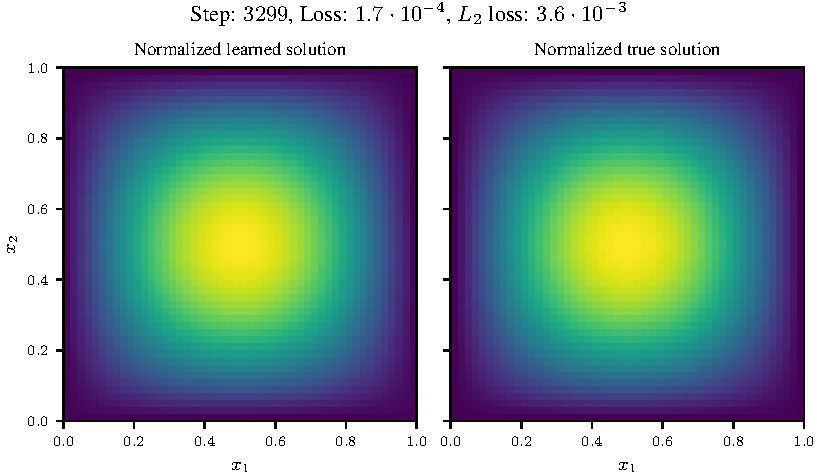
\includegraphics[scale=2,trim={0.9cm 0.8cm 6.7cm 1cm}, clip]{../kfac_pinns_exp/exp42_visualize_solutions/visualize_solution/SGD/poisson_2d_sin_product_mlp-tanh-64_SGD_step0003299.pdf}

      \textbf{Trained}
    \end{minipage}
    \hfill
    \begin{minipage}{0.33\linewidth}
      \centering
      % [trim={left bottom right top},clip]
      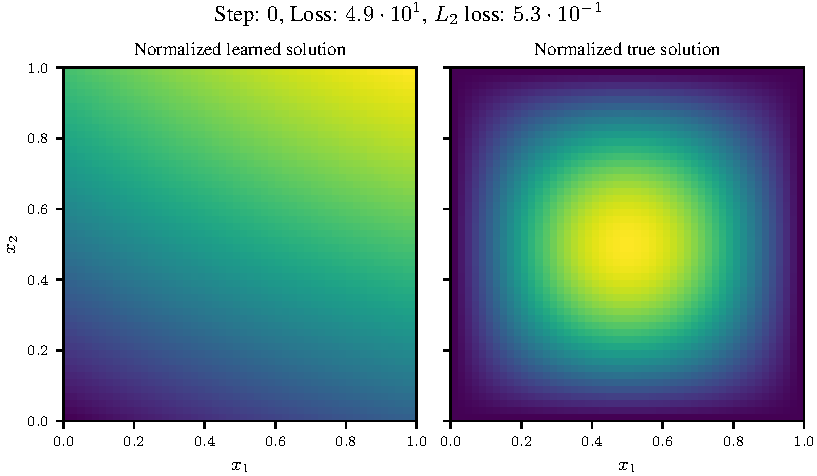
\includegraphics[scale=2,trim={7.3cm 0.8cm 0.1cm 1cm}, clip]{../kfac_pinns_exp/exp42_visualize_solutions/visualize_solution/SGD/poisson_2d_sin_product_mlp-tanh-64_SGD_step0000000.pdf}

      \textbf{True solution}
    \end{minipage}
  }

  \column{0.9}
  \block{Contribution: How Do We Derive KFAC for PINN Losses?}{
    \begin{center}
      \begin{Large}
        \textcolor{VectorBlue}{\textbf{We show that computing differential operators with Taylor-mode autodiff yields networks with linear weight sharing layers}
        \\[0.5ex]
        $\mathbf{\to}$ \textbf{This allows us to apply the existing definition of KFAC for linear weight sharing layers.}}
      \end{Large}
    \end{center}

    \begin{minipage}{0.3\linewidth}

      \vspace{2ex}

      \begin{itemize}
      \item \textbf{Goal:} Approximate Gauss-Newton matrix
        \begin{align*}
          \mG(\mW) = \mG_{\Omega}(\mW) + \mG_{\partial \Omega}(\mW)
        \end{align*}
        for each linear layer with weight $\mW$
        \begin{align*}
          \mG_{\Omega}(\mW)
          &\approx
            \mA_{\Omega} \otimes \mB_{\Omega}
          \\
          \mG_{\partial\Omega}(\mW)
          &\approx
            \mA_{\partial\Omega} \otimes \mB_{\partial\Omega}
        \end{align*}

        \vspace{0.7ex}

      \item \textbf{Contribution:} Make computation of $L(\vtheta)$ explicit
        \begin{itemize}
        \item Linear layer in boundary loss
          \begin{align*}
            \vz \mapsto \mW \vz \qquad \textbf{($\vz$ is a vector)}
          \end{align*}
        \item Linear layer in interior loss
          \begin{align*}
            \mZ \mapsto \mW \mZ \qquad \textbf{($\mZ$ is a matrix)}
          \end{align*}
        \end{itemize}
      \end{itemize}

      \vspace{2ex}

      \textbf{The computation reduces to a neural net with linear weight sharing layers.
        We can just apply the existing KFAC definition from Eschenhagen (NeurIPS 2023).}
    \end{minipage}
    \hfill
    \begin{minipage}{0.68\linewidth}
      \centering
      \hspace{-13.25ex}% Define styles of nodes in computation graph sketch
\tikzset{%
  % shared basic style
  basicNode/.style={%
    rectangle,%
    minimum width=5ex,%
    minimum height=3.5ex,%
    inner sep=0.3ex,%
    rounded corners,%
    draw=black,%
    thick,%
    fill opacity=0.3,%
    text opacity=1.0,%
  },%
  % style for nodes representing neural network parameters
  paramNode/.style={%
    basicNode,%
    fill=maincolor,%
  },%
  % style for nodes representing data
  inputNode/.style={%
    basicNode,%
    fill=secondcolor,%
  },%
  % style for nodes indicating a repetition
  dotsNode/.style={%
    basicNode,%
    draw opacity=0,%
  },%
  % style for nodes representing intermediates from the forward pass
  forwardNode/.style={%
    basicNode,%
    fill=thirdcolor,%
  },%
  % style for nodes representing intermediates from the gradient backpropagation
  gradientNode/.style={%
    basicNode,%
    fill=fourthcolor,%
  },%
  % style for nodes representing intermediates from the Hessian % backpropagation
  hessianNode/.style={%
    basicNode,%
    fill=fifthcolor,%
  },%
}%
%%% Local Variables:
%%% mode: latex
%%% TeX-master: "../main"
%%% End:

\colorlet{maincolor}{VectorPink}
\colorlet{secondcolor}{VectorOrange}
\colorlet{thirdcolor}{VectorTeal}
\colorlet{fourthcolor}{white}
\colorlet{fifthcolor}{red}
\begin{tikzpicture}
  % arrange nodes in a matrix
  \matrix [%
  row sep=3.25ex,%
  column sep=4.5ex,%
  ampersand replacement=\&,% in order to put this inside of a scalebox
  ]{%
    % neural network parameters
    \&
    \node [paramNode] (param-1) {$\mW^{(1)}$};
    \&
    \node [dotsNode] (param-2) {$\dots$};
    \&
    \node [paramNode] (param-3) {$\mW^{(i-1)}$};
    \&
    \node [paramNode] (param-4) {$\mW^{(i)}$};
    \&
    \node [dotsNode] (param-5) {$\dots$};
    \&
    \node [paramNode] (param-6) {$\mW^{(L)}$};
    \\
    % forward pass
    \node [inputNode] (forward-0) {$\vx$};
    \&
    \node [forwardNode] (forward-1) {$\vz^{(1)}$};
    \&
    \node [dotsNode] (forward-2) {$\dots$};
    \&
    \node [forwardNode] (forward-3) {$\vz^{(i-1)}$};
    \&
    \node [forwardNode] (forward-4) {$\vz^{(i)}$};
    \&
    \node [dotsNode] (forward-5) {$\dots$};
    \&
    \node [forwardNode] (forward-6) {$u(\vx)$};
    \\
  };
  % dependency arrows
  \foreach \i in {1,...,6} {
    \draw [-Latex, line width=4pt, VectorBlue] (param-\i) to (forward-\i);
  }
  \foreach \i in {0,...,5} {
    \pgfmathsetmacro{\j}{int(\i+1)}
    \draw [-Latex, line width=3pt] (forward-\i) to (forward-\j);
  }
\end{tikzpicture}
%%% Local Variables:
%%% mode: latex
%%% TeX-master: "../main"
%%% End:


      \textbf{Boundary loss compute graph}

      \vspace{2ex}

      % Define styles of nodes in computation graph sketch
\tikzset{%
  % shared basic style
  basicNode/.style={%
    rectangle,%
    minimum width=5ex,%
    minimum height=3.5ex,%
    inner sep=0.3ex,%
    rounded corners,%
    draw=black,%
    thick,%
    fill opacity=0.3,%
    text opacity=1.0,%
  },%
  % style for nodes representing neural network parameters
  paramNode/.style={%
    basicNode,%
    fill=maincolor,%
  },%
  % style for nodes representing data
  inputNode/.style={%
    basicNode,%
    fill=secondcolor,%
  },%
  % style for nodes indicating a repetition
  dotsNode/.style={%
    basicNode,%
    draw opacity=0,%
  },%
  % style for nodes representing intermediates from the forward pass
  forwardNode/.style={%
    basicNode,%
    fill=thirdcolor,%
  },%
  % style for nodes representing intermediates from the gradient backpropagation
  gradientNode/.style={%
    basicNode,%
    fill=fourthcolor,%
  },%
  % style for nodes representing intermediates from the Hessian % backpropagation
  hessianNode/.style={%
    basicNode,%
    fill=fifthcolor,%
  },%
}%
%%% Local Variables:
%%% mode: latex
%%% TeX-master: "../main"
%%% End:

\colorlet{maincolor}{VectorPink}
\colorlet{secondcolor}{VectorOrange}
\colorlet{thirdcolor}{VectorTeal}
\colorlet{fourthcolor}{white}
\colorlet{fifthcolor}{red}
\begin{tikzpicture}
  % arrange nodes in a matrix
  \matrix [%
  row sep=3.25ex,%
  column sep=4.5ex,%
  ampersand replacement=\&,% in order to put this inside of a scalebox
  ]{%
    % neural network parameters
    \&
    \node [paramNode] (param-1) {$\mW^{(1)}$};
    \&
    \node [dotsNode] (param-2) {$\dots$};
    \&
    \node [paramNode] (param-3) {$\mW^{(i-1)}$};
    \&
    \node [paramNode] (param-4) {$\mW^{(i)}$};
    \&
    \node [dotsNode] (param-5) {$\dots$};
    \&
    \node [paramNode] (param-6) {$\mW^{(L)}$};
    \\
    % forward pass
    \node [inputNode] (forward-0) {$\vx$};
    \&
    \node [forwardNode] (forward-1) {$\vz^{(1)}$};
    \&
    \node [dotsNode] (forward-2) {$\dots$};
    \&
    \node [forwardNode] (forward-3) {$\vz^{(i-1)}$};
    \&
    \node [forwardNode] (forward-4) {$\vz^{(i)}$};
    \&
    \node [dotsNode] (forward-5) {$\dots$};
    \&
    \node [forwardNode] (forward-6) {$u(\vx)$};
    \\
    % gradients
    \node [inputNode] (gradient-0) {$\mI_d$};
    \&
    \node [gradientNode] (gradient-1) {$\partial_{\vx}\vz^{(1)}$};
    \&
    \node [dotsNode] (gradient-2) {$\dots$};
    \&
    \node [gradientNode] (gradient-3) {$\partial_{\vx}\vz^{(i-1)}$};
    \&
    \node [gradientNode] (gradient-4) {$\partial_{\vx}\vz^{(i)}$};
    \&
    \node [dotsNode] (gradient-5) {$\dots$};
    \&
    \node [gradientNode] (gradient-6) {$\partial_{\vx}u(\vx)$};
    \\
    % Hessians
    \node [inputNode] (hessian-0) {$\vzero_{d\times d}$};
    \&
    \node [hessianNode] (hessian-1) {$\partial^2_{\vx} \vz^{(1)}$};
    \&
    \node [dotsNode] (hessian-2) {$\dots$};
    \&
    \node [hessianNode] (hessian-3) {$\partial^2_{\vx}\vz^{(i-1)}$};
    \&
    \node [hessianNode] (hessian-4) {$\partial^2_{\vx}\vz^{(i)}$};
    \&
    \node [dotsNode] (hessian-5) {$\dots$};
    \&
    \node [hessianNode] (hessian-6) {$\partial^2_{\vx}u(\vx)$};
    \&
    \node [hessianNode] (hessian-7) {$\gL u(\vx)$};
    \\
  };
  % dependency arrows
  \foreach \i in {1,...,6} {
    \draw [-Latex, line width=4pt, VectorBlue] (param-\i) to (forward-\i);
  }
  \foreach \i in {0,...,5} {
    \pgfmathsetmacro{\j}{int(\i+1)}
    \draw [-Latex, line width=3pt] (forward-\i) to (forward-\j);
    \draw [-Latex, line width=3pt] (gradient-\i) to (gradient-\j);
    \draw [-Latex, line width=3pt] (hessian-\i) to (hessian-\j);
  }
  \foreach \i in {1,...,6} {
    \draw [-Latex, line width=4pt, VectorBlue, out=215, in=135] (param-\i) to (gradient-\i);
    \draw [-Latex, line width=4pt, VectorBlue, out=215, in=135] (param-\i) to (hessian-\i);
  }
  \draw [-Latex, line width=3pt] (hessian-6) to (hessian-7);
  \draw [-Latex, line width=3pt, out=315, in=135] (gradient-6) to (hessian-7);
  \draw [-Latex, line width=3pt, out=315, in=90] (forward-6) to (hessian-7);
\end{tikzpicture}
%%% Local Variables:
%%% mode: latex
%%% TeX-master: "../main"
%%% End:


      \textbf{Interior loss compute graph} (simplified)

    \end{minipage}
  }
\end{columns}

\begin{columns}
  \column{0.9}
  \block{Motivation: PINNs Are Hard to Train, Second-order Methods Can Help}{
    \begin{center}
      \begin{Large}
        \textcolor{VectorBlue}{\textbf{Second-order methods beat first-order methods on small problems\dots
          but do not scale well to larger nets $\mathbf{\to}$ our KFAC scales.}}
      \end{Large}
    \end{center}

    \hfill
    \begin{minipage}{0.08\linewidth}
      \textbf{Small net}
      \\
      \textbf{($\mathbf{D = 257}$)}
    \end{minipage}
    \begin{minipage}{0.38\linewidth}
      \centering
      % [trim={left bottom right top},clip]
      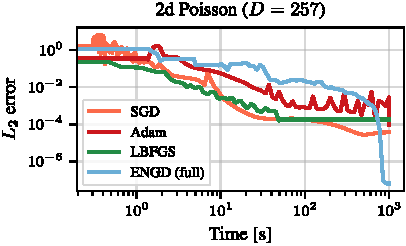
\includegraphics[width=0.85\linewidth, trim={0 0 0 0.3cm},clip]{../presentation/figures/poisson2d-02.pdf}
    \end{minipage}
    \hfill
    \begin{minipage}{0.38\linewidth}
      \centering
      % [trim={left bottom right top},clip]
      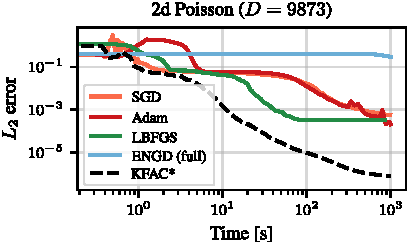
\includegraphics[width=0.85\linewidth, trim={0 0.08cm 0 0.3cm},clip]{figures/poisson2d-medium.pdf}
    \end{minipage}
    \begin{minipage}{0.08\linewidth}
      \textbf{Medium net}
      \\
      \textbf{($\mathbf{D = 9873}$)}
    \end{minipage}
    \hfill
  }
  \column{0.9}
  \block{Evaluation: Our KFAC Optimizer Outperforms First-order Methods and Scales Well}{
    \begin{minipage}[t]{0.31\linewidth}
      \centering
      \textbf{9+1d log-Fokker-Planck equation, $\mathbf{D \approx 10^5}$}

      \vspace{1ex}

      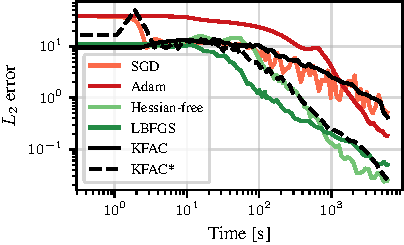
\includegraphics[width=\linewidth]{../kfac_pinns_exp/exp43_log_fokker_planck9d_isotropic_gaussian_random/l2_error_over_time.pdf}
    \end{minipage}
    \hfill
    \begin{minipage}[t]{0.28\linewidth}
      \centering
      \textbf{4+1d Heat equation, $\mathbf{D \approx 10^5}$}

      % [trim={left bottom right top},clip]
      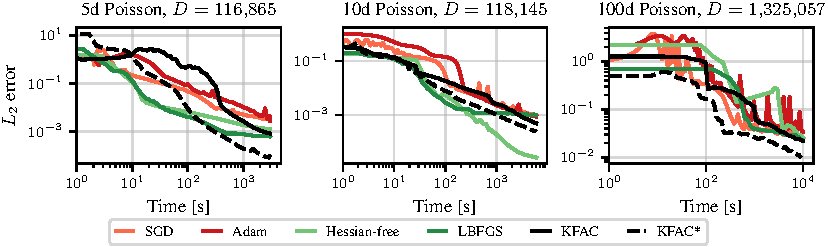
\includegraphics[trim={9.5cm 0.5cm 0 0.3cm},clip, width=0.93\linewidth]{../kfac_pinns_exp/exp33_poisson_bayes_groupplot/l2_error_over_time.pdf}
    \end{minipage}
    \hfill
    \begin{minipage}[t]{0.28\linewidth}
      \centering
      \textbf{100d Poisson equation, $\mathbf{D\approx 10^6}$}

      % [trim={left bottom right top},clip]
      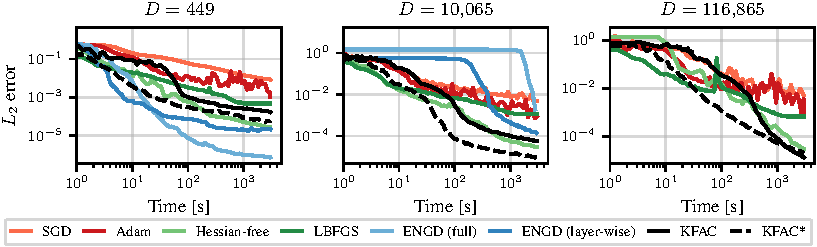
\includegraphics[trim={9.5cm 0.5cm 0 0.3cm},clip, width=0.9\linewidth]{../kfac_pinns_exp/exp30_heat4d_groupplot/l2_error_over_time.pdf}
    \end{minipage}
    \hfill

    \vspace{-0.5ex}
  }
\end{columns}

\end{document}
%%% Local Variables:
%%% mode: LaTeX
%%% TeX-master: t
%%% End:
